\count\Afootins=1200
\count\Bfootins=1200
\count\Cfootins=1200
\pstart \edtext{Instrumenta metallina}{\lemma{Instrumenta}\Bfootnote{\textit{(1)}\ lignea \textit{(2)}\ metallina \textit{L}}}\protect\index{Sachverzeichnis}{instrumenta metallina}, nisi bene fortificata facilius curvantur, quam lignea crassa. Itaque ut maneant semper plana ponenda super tabula lignea vel forma \edtext{(\textit{frame})}{\lemma{\hspace{-0.5mm}(\textit{frame})}\Cfootnote{a.a.O., S. 18.\hspace{-3mm}}} fortificata contra curvationes, et in variis instrumenti partibus ope exiguarum cochlearum affirmanda ligno, tota interim \edtext{tabula aequilibrata}{\lemma{tabula}\Bfootnote{\textit{(1)}\ contre baton \textit{(2)}\ aequilibrata \textit{L}}}, ut facilius moveatur.
\pend 
\pstart Pro divisione per diagonales tandem elegit Hevelius\protect\index{Namensregister}{\textso{Hevelius}, Johannes (1611-1687)} divisionem aliam de qua scripsit Hedraeus\protect\index{Namensregister}{\textso{Hedraeus}, Bengt (1608-1659)}. Nempe Hevelius\protect\index{Namensregister}{\textso{Hevelius}, Johannes (1611-1687)} quadrantem\protect\index{Sachverzeichnis}{quadrans} facit non graduum 90 sed 110. pro habendis divisionibus cujuslibet gradus quadrantis\protect\index{Sachverzeichnis}{quadrans} ope \textit{of a new invented perpendicular of} \edtext{\textit{brass}}{\lemma{\hspace{-0.5mm}\textit{brass}}\Cfootnote{a.a.O., S. 20.\hspace{-3mm}}}. Putat Hedraeum\protect\index{Namensregister}{\textso{Hedraeus}, Bengt (1608-1659)} non esse inventorem, sed ex observatorio vel potius Repositorio Tychonis\protect\index{Namensregister}{\textso{Brahe}, Tycho (1546-1601)} habuisse. Erravere Hedraeus\protect\index{Namensregister}{\textso{Hedraeus}, Bengt (1608-1659)} et Hevelius\protect\index{Namensregister}{\textso{Hevelius}, Johannes (1611-1687)} quod credidere diagonales geometricae exactitudinis incapaces. Imo contra, diagonalis linea semper est pars tangentis, hoc est spatia inter parallelos circulos debent semper esse, \textit{in proportion to the difference of some tangent lines and the different distance of those circles from the center are alwayes to be in proportion of the difference of some tangent lines, and the different distance of those circles from the center}   
\textit{are alway in proportion of some} \edtext{\textit{secants:}}{\lemma{\hspace{-0.5mm}\textit{secants:}}\Cfootnote{a.a.O., S. 21.\hspace{-3mm}}} \edtext{Tycho}{\lemma{\textit{secants:}}\Bfootnote{\textit{(1)}\ \textit{and the way of f} \textit{(2)}\ Hevelius \textit{(3)}\ Tycho \textit{L}}} in \edtext{fine \textit{Mechanicorum}}{\lemma{\hspace{-0.5mm}fine \textit{Mechanicorum}}\Cfootnote{\textsc{T. Brahe}, \textit{Astronomiae instauratae mechanica}, Wandesburg 1598 (nicht paginiert), Abschnitt \glqq Supplementum de subdivisione et dioptris instrumentorum\grqq~beginnend auf der drittletzten Seite (\textit{TBO} V, S. 153-155).}} demonstrat errorem esse perexiguum diagonalium etiam interstitiorum aequalium. Sed facillime vera et naturalis habetur divisio, si proponatur $BC$ repraesentare diagonalem lineam subtendentem angulum 10' ad centrum $A$. Producatur linea $BC$ ad $F$, et cadat perpendicularis a centro $A$ ad $E$. Supponatur angulus ad $B$ unius gradus erit $BE$ tangens graduum 89. radio posito $AE$. Et $EC$ tangens \edtext{\textit{88,50'}}{\lemma{\textit{88,50'}}\Cfootnote{\textsc{R. Hooke}, \textit{Animadversions}, S. 23.}} et differentiae tangentium \textit{88,50'. 88,51'. 88,52' 88,53'. 88,54'. 88,55'. 88,56'. 88,57'. 88,58'.} \edtext{\textit{88,59' et 89.}}{\lemma{\textit{88,59' et 89.}}\Cfootnote{a.a.O., S. 23.}} dant distantias circulorum: \textit{C. 1. 2. 3. 4. 5. 6. 7. 8. 9.} \edtext{\textit{B}}{\lemma{\textit{B}}\Cfootnote{a.a.O., S. 23.}} (NB. non posui omnes numeros in figura.) Alia \edtext{methodo intervalla}{\lemma{methodo}\Bfootnote{\textit{(1)}\ haec \textit{(2)}\ intervalla \textit{L}}} assignat Hevelius\protect\index{Namensregister}{\textso{Hevelius}, Johannes (1611-1687)} ingeniosa et accurata. Aliam methodum continet Wallisius\protect\index{Namensregister}{\textso{Wallis}, John (1616-1703)} in Epistola ad Hevelium\protect\index{Namensregister}{\textso{Hevelius}, Johannes (1611-1687)}, quam inseruit Hookius\protect\index{Namensregister}{\textso{Hooke}, Robert (1635-1703)} dissertationi suae, sed non videtur ita expedita. 
\pend 
\newpage
\pstart
\noindent
\begin{wrapfigure}[17]{l}{0.44\textwidth}   
\vspace{-8mm}                 
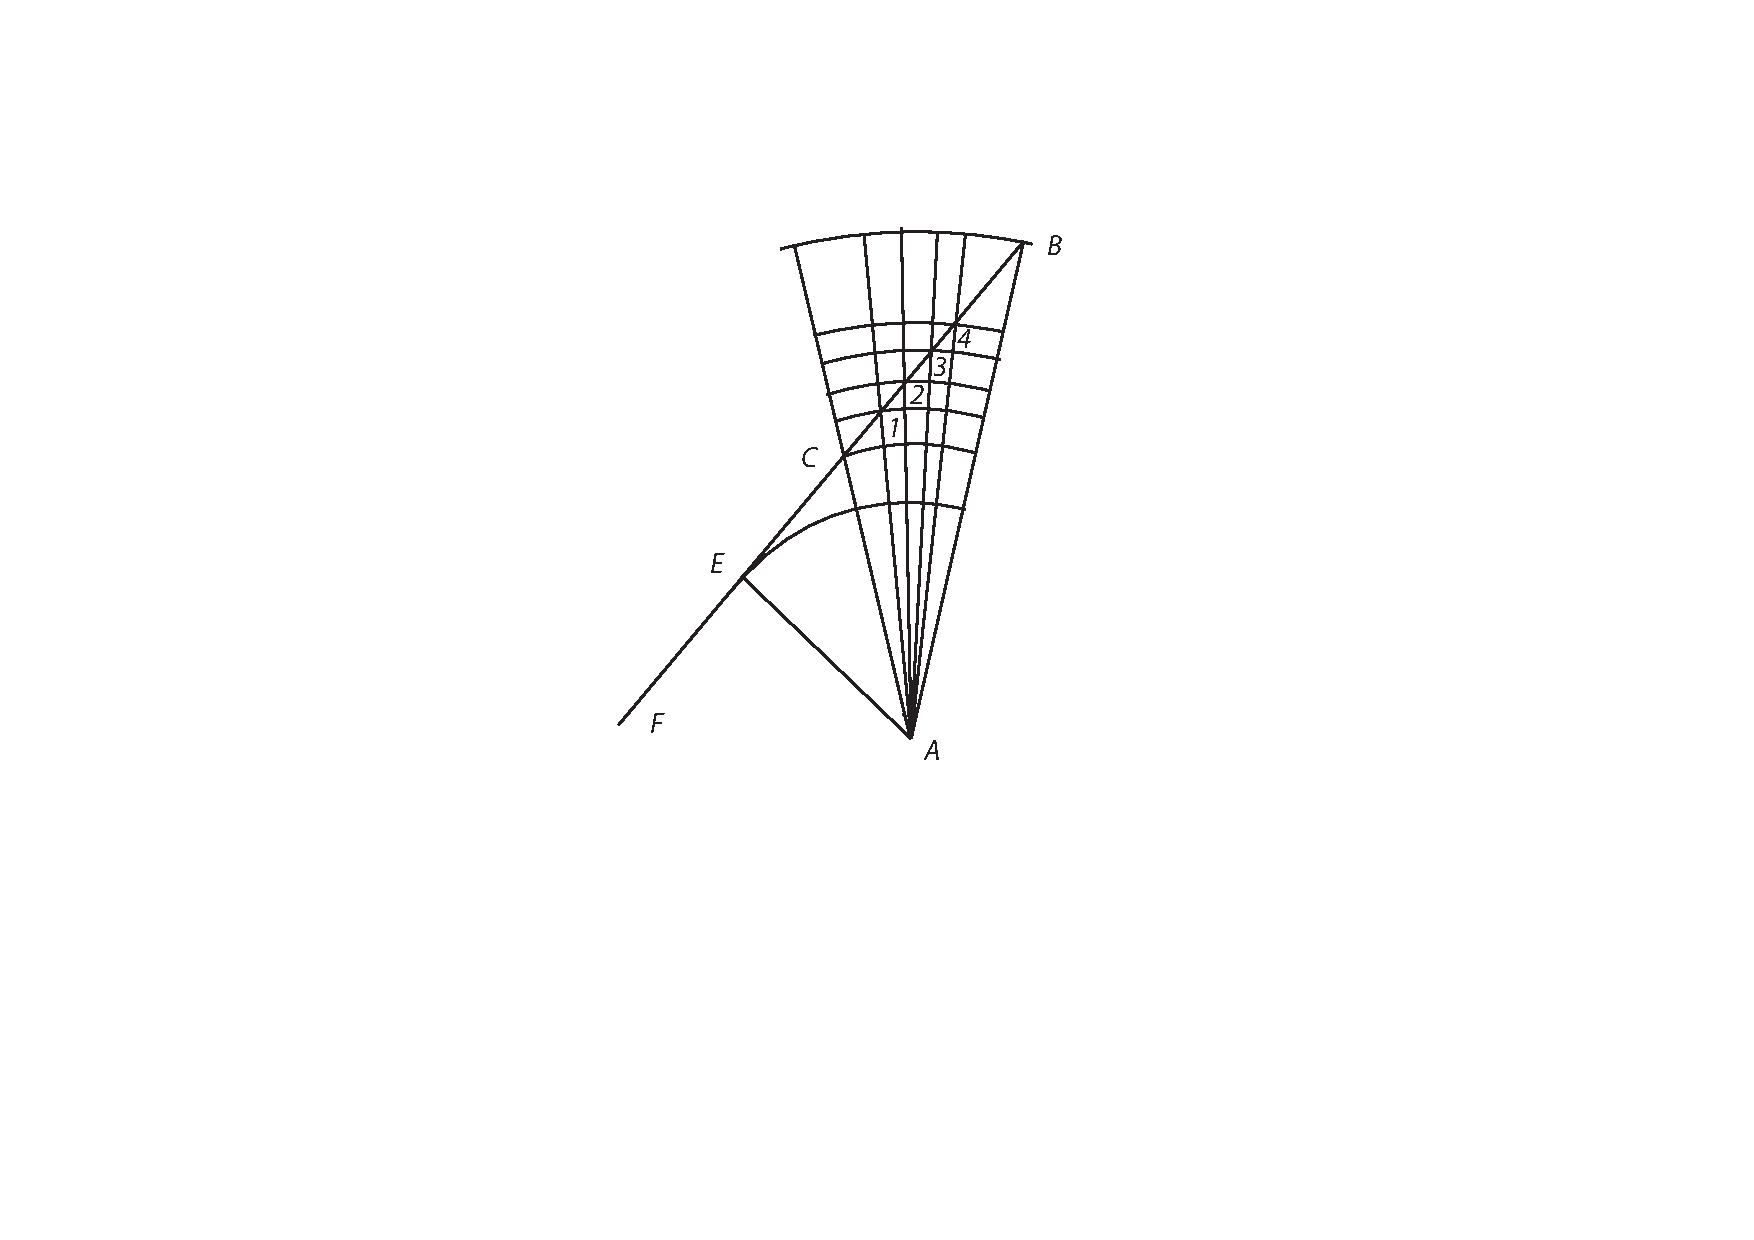
\includegraphics[trim = 0mm 2mm 0mm 0mm, clip, width=0.44\textwidth]{images/lh0351506_11r-d1.pdf}\\
\centering \rule[0pt]{0mm}{0pt}[\textit{Fig. 2, nach Hooke Fig. 35}]
\end{wrapfigure}
\textit{Pierre Vernier}\protect\index{Namensregister}{\textso{Vernier}, Pierre (1580-1635)} \textit{Capitain et chastelain pour sa Mt\'{e}}\protect\index{Namensregister}{\textso{Philipp III. K\"{o}nig von Spanien (1598-1621)}, Philipp IV. K\"{o}nig von Spanien (1621-1665)} \textit{au chasteau Dornans}\protect\index{Ortsregister}{Ornans} \textit{Conseiller et General de ses monnoyes au Comt\'{e} de} \edtext{\textit{Bourgogne}\protect\index{Ortsregister}{Burgund}}{\lemma{\textit{Bourgogne}}\Cfootnote{a.a.O., S. 30.}} \`{a} Brusselles\protect\index{Ortsregister}{Br\"{u}ssel} chez Fran\c{c}ois Vivien\protect\index{Namensregister}{\textso{Vivien}, Fran\c{c}ois}. Le titre du \edtext{liure}{\lemma{liure}\Cfootnote{\textsc{P. Vernier}, \textit{La Construction, l'usage et les propri\'{e}tez du quadrant\protect\index{Sachverzeichnis}{quadrans} nouveau de math\'{e}matique}, Br\"{u}ssel 1631.}} est: \textit{La construction l'usage et les proprietez du quadrant\protect\index{Sachverzeichnis}{quadrans} 
nouueau mathematique, comme aussi la construction de la table des sinus de minute en minutes successivement par une seule maxime. 
De plus un abreg\'{e} des dites tables en une petite demy-page, avec son usage, et en fin la methode de trouuer les angles d'un triangle par la connoissance des costez, et les costez par les angles, sans aide d'aucune Table}.
\\
\indent
Methodus descripta a Hookio pro faciendo catalogo fixarum accuratissimo vix decima laboris parte et temporis, et multo exactius: Fiat largus quadrans muralis vel potius semicirculus radii triginta pedum fixus exacte in meridiano\protect\index{Sachverzeichnis}{meridian} in muro ex quadratis lapidibus, bene junctis \textit{and cramped together,}\edtext{}{\lemma{\textit{together},}\Cfootnote{\cite{00332}\textsc{R. Hooke}, \textit{Animadversions}, S. 32.}} et positis super fundamento, firmo et solido \textit{to prevent all manner of slacking and swarfing. The rim of his}\edtext{}{\lemma{\textit{his}}\Cfootnote{a.a.O., S. 32.}} sit ex laminis aeneis in debito situ locatis ope ferreorum (barres) baculorum in muro fixorum, \textit{by running them with lead}\edtext{}{\lemma{\textit{lead}}\Cfootnote{a.a.O., S. 32.}} (+ cum plumbo infuso). Diviso hoc semicirculo in 180 gradus, et subdiviso quolibet gradu ope diagonalium super bene polita vitri tabula, divisa per minuta et secunda modo supra descripto: his factis adaptetur et Telescopium\protect\index{Sachverzeichnis}{telescopium} triginta pedum, ita ut Tubus non curvetur, nec vitrum excedat vero situ. Focus vitri objectivi sit \edtext{exacte \textit{upon the edge}}{\lemma{exacte}\Bfootnote{\textit{(1)}\ super uno edge \textit{(2)}\ \textit{upon the edge} \textit{L}}} (acies) \textit{of the brass limb,}\edtext{}{\lemma{\textit{limb,}}\Cfootnote{a.a.O., S. 32.}} limbi aenei ita ut ope ocularis\protect\index{Sachverzeichnis}{ocular}, quod est \textit{a deep convex}\edtext{}{\lemma{\textit{convex}}\Cfootnote{a.a.O., S. 32.}} punctualis locus vel altitudo stellae ad quartam pili latitudinis partem possit observari. Impedimentum curvaturae Telescopii\protect\index{Sachverzeichnis}{telescopium} fieri potest eo fere modo quem communicavi Hevelio\protect\index{Namensregister}{\textso{Hevelius}, Johannes (1611-1687)}, et \edtext{quem descriptum}{\lemma{}\Bfootnote{quem \textbar\ large \textit{gestr.}\ \textbar\ descriptum \textit{L}}} invenies apud ipsum. Excepto quod \edtext{\textit{instead of Ropes}}{\lemma{\textit{instead of Ropes}}\Cfootnote{a.a.O., S. 33.}} (loco restium) nunc commendo totidem braces (fibulas armillas) ligneas. Et licet non obstante omni diligentia evitari nequeat ut tubus in medio nonnihil curvetur, sed hoc non vitiabit observationem, quia vitrum objectivum eundem semper situm servat ad centrum, et focus ejus est exacte \edtext{\textit{in the edge of the limb}}{\lemma{\textit{limb}}\Cfootnote{a.a.O., S. 33.}}. Inconvenientia respiciendi \edtext{sursum inque}{\lemma{sursum}\Bfootnote{\textit{(1)}\ in lim \textit{(2)}\ inque \textit{L}}} alio \edtext{situ incommodo}{\lemma{situ}\Bfootnote{\textit{(1)}\ indebito \textit{(2)}\ incommodo \textit{L}}} \edtext{[praevenietur]}{\lemma{}\Bfootnote{prevenietur \textit{L \"{a}ndert Hrsg.}}} ope reflexi metalli cujus ope semper respicietur horizontaliter, hoc est perpendiculariter ad planum muri vel quadrantis\protect\index{Sachverzeichnis}{quadrans}. Et ut praeveniatur labor movendi (ope longi ligni) \edtext{ope \textit{of}}{\lemma{}\Bfootnote{ope \textit{of} \textit{erg. L}}} \textit{a long yard poysed upon centers on a frame before the said instrument}\edtext{}{\lemma{\textit{instrument}}\Cfootnote{a.a.O., S. 33.}}. Tubus brachium cum dioptra\protect\index{Sachverzeichnis}{dioptra} et sedes observatoris cui insidet simul possunt esse aequilibrata, ita ut circumagendo a \edtext{\textit{Windle,}}{\lemma{\textit{Windle},}\Cfootnote{a.a.O., S. 33.\hspace{15mm}}} facile sit movere se ad ullum situm desideratum. Objectivum est exacte ante centrum, et oculare\protect\index{Sachverzeichnis}{ocular} directe respicit divisiones limbi. Hac ratione observationes unius noctis sumi possunt aliquot centenarum \edtext{stellarum declinationes\protect\index{Sachverzeichnis}{declinationes stellarum}}{\lemma{stellarum}\Bfootnote{\textit{(1)}\ observat \textit{(2)}\ declinationes \textit{L}}} ad secundum usque minutum, modo sint \edtext{duo}{\lemma{}\Bfootnote{duo \textit{erg.} \textit{L}}} assistentes qui notent quae vides. Et eodem tempore recta ascensio cujuslibet eorum sumi potest, ope horologii penduli circularis: \textit{a accurate compound circular \textso{pendulums-clock\protect\index{Sachverzeichnis}{pendulum-clock}}},\edtext{}{\lemma{\textit{\textso{pendulums-clock}},}\Cfootnote{a.a.O., S. 33.}} quod alias describam notans ad secundum usque minutum appulsum cujusque stellae ad meridianum\protect\index{Sachverzeichnis}{meridian}, cumque objici posset refractione aeris variaturas declinationes earum stellarum\protect\index{Sachverzeichnis}{declinationes stellarum} quae \edtext{sunt meridionales}{\lemma{sunt}\Bfootnote{\textit{(1)}\ in ax \textit{(2)}\ meridionales \textit{L}}} valde, attamen cum hoc instrumentum viam suppeditet supra aliud quod sit in mundo, pro detegendis diversis refractionibus \edtext{aeris pro variis supra horizontem altitudinibus, usque ad secundi}{\lemma{aeris}\Bfootnote{\textit{(1)}\ ad sec \textit{(2)}\ pro [...] secundi \textit{L}}} exactitudinem sumendo altitudinem harum stellarum \textit{as never set in the North}\edtext{}{\lemma{\textit{North}}\Cfootnote{a.a.O., S. 34.}} in maxima et minima altitudine supra horizontem; Tabula harum refractionum facile rectificabit declinationem aliarum fixarum ad magnam altitudinem. 
\pend 
\count\Afootins=1200
\count\Bfootins=1200
\count\Cfootins=1200
\pstart Ad instrumentum\protect\index{Sachverzeichnis}{instrumentum Hevelii} Hevelii\protect\index{Namensregister}{\textso{Hevelius}, Johannes (1611-1687)} quo altitudines \edtext{meridianis\protect\index{Sachverzeichnis}{meridian} sumere praetendit}{\lemma{meridianis}\Bfootnote{\textit{(1)}\ sumit \textit{(2)}\ sumere praetendit \textit{L}}} ad secundum usque minutum, \edtext{respondet Hookius}{\lemma{respondet}\Bfootnote{\textit{(1)}\ Hevelius \textit{(2)}\ Hookius \textit{L}}} secundum minutum in eo instrumento esse ter millesimam pollicis partem quam nudus visus discernere nequeat et aegre Microscopio adjutus. Sed quomodo inquit discernet penumbram\protect\index{Sachverzeichnis}{penumbra}, quae non est certa ad minutum usque. Et quanquam dici queat, \textit{it is the same, round the circle, and the circle is the true bigness of the sun,}\edtext{}{\lemma{\textit{sun},}\Cfootnote{a.a.O., S. 35.}} ita ut circulus magnitudinis respondentis diametro solis\protect\index{Sachverzeichnis}{diametrus solis} et distantiae inferioris dioptrae\protect\index{Sachverzeichnis}{dioptra} a superiori, super ipsa inferiore describatur necesse esse [11~v\textsuperscript{o}]